
\documentclass{article}
\usepackage{graphicx} % Required for inserting images
\usepackage[utf8]{inputenc}
\usepackage{amsmath}
\usepackage{graphicx}
\graphicspath{{images/}}
\usepackage{float}
\title{Deep CNN for Garbage Classification}
\author{Samuele Magatti}

\begin{document}

\maketitle


\section{Introduction}
In this project, I implement a Deep Neural Network for image classification using the Garbage dataset.


\section{Dataset}


Before running the code be sure to have the kaggle.json file with your kaggle credentials aviable on your computer, refer to the instructions contained in the readme file for more information. 
The dataset analysis pipeline first verifies that the dataset has been
correctly downloaded and inspects its structure. The dataset provides
three versions of the images: one with non-standardized images and two
with standardized images. This project uses the standardized images
with a resolution of 256 × 256 pixels contained in the
`standardized 256` folder.


\section{Dataset audit}

 The dataset is divided in ten classes:  biological, battery, cardboard, paper, metal, shoes, clothes, plastic, trash and glass.
 The classes are not equally distributed, as shown in Figure
1. The imbalance ratio is equal to 4.19.
Consequently, all subsequent splits and subsamples of the dataset are performed using stratified sampling.


\begin{figure}[H]
    \centering
    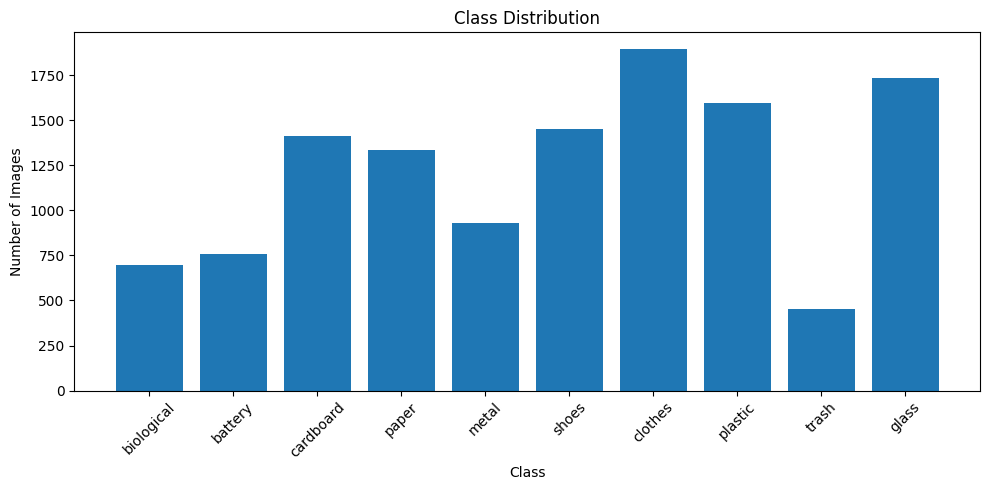
\includegraphics[width=0.8\textwidth]{images/class_distribution_garbage_cnn.png}
    \caption{Distribution of the images among the ten garbage classes.}
    \label{fig:class_distribution}
\end{figure}


The audit pipeline also checks for corrupted and duplicated images.
Duplicate detection is performed through image hashing in order to
maintain a reasonable execution time. No corrupted or duplicated
images were found.


\section{Data Organization}

In order to prioritize the running time the dataset has been subsampled using a stratified subsample that reduced the total number of images used to 3016, a quarter of the initial dataset total amount of images. the following table will show how the images are distributed between the classes in the full dataset and in the subsample, no significant difference can be spotted. The following image will show instead the proportion of each class that will be used in the dataset compared with the previous distribution.


\begin{table}[H]
\centering
\caption{Class proportions in the original dataset and in the stratified subsample.}
\label{tab:stratified_subsample}
\begin{tabular}{lcc}
\hline
Class & Full Dataset & Subsample \\
\hline
Clothes    & 0.1543 & 0.1544 \\
Glass      & 0.1416 & 0.1416 \\
Plastic    & 0.1303 & 0.1302 \\
Shoes      & 0.1182 & 0.1181 \\
Cardboard  & 0.1151 & 0.1152 \\
Paper      & 0.1090 & 0.1090 \\
Metal      & 0.0759 & 0.0757 \\
Battery    & 0.0617 & 0.0617 \\
Biological & 0.0570 & 0.0571 \\
Trash      & 0.0369 & 0.0369 \\
\hline
\end{tabular}
\end{table}

\begin{figure}[h]
    \centering
    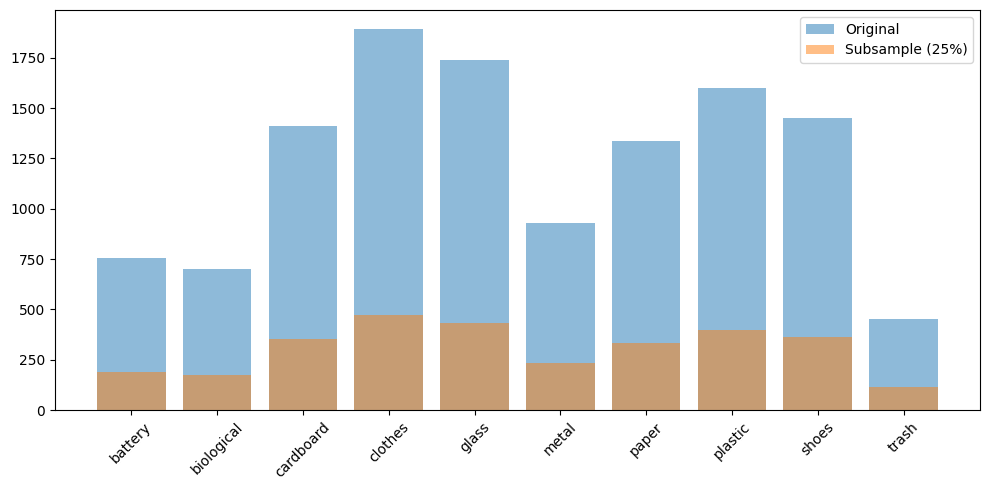
\includegraphics[width=0.8\textwidth]{images/subsample.labels.garbage.dnn.png}
    \caption{Distribution of the images among the ten garbage classes.}
    \label{fig:subsample_class_distribution}
\end{figure}






\section{Pre-processing}


The dataset was divided into training and test sets using a stratified train-test split. The training set contains approximately 80\% of the observations, while the remaining 20\% constitute the test set.
The following table will show that no significant difference can be found between the original dataset and the train and test class distribution.

\begin{table}[h]
\centering
\caption{Class proportions in the train and test sets after the stratified split.}
\label{tab:train_test_split}
\begin{tabular}{lccc}
\hline
Class & Train & Test & Difference \\
\hline
Clothes   & 0.1542 & 0.1550 & 0.0008 \\
Glass     & 0.1416 & 0.1419 & 0.0004 \\
Plastic   & 0.1302 & 0.1305 & 0.0004 \\
Shoes     & 0.1183 & 0.1175 & 0.0009 \\
Cardboard & 0.1151 & 0.1158 & 0.0008 \\
Paper     & 0.1089 & 0.1093 & 0.0004 \\
Metal     & 0.0759 & 0.0750 & 0.0008 \\
Battery   & 0.0616 & 0.0620 & 0.0004 \\
Biological& 0.0571 & 0.0571 & 0.0000 \\
Trash     & 0.0371 & 0.0359 & 0.0012 \\
\hline
\end{tabular}
\end{table}


To do the hyperparameters selection the dataset is divided in 3 folds and the train validation structure, in witch each part contained two folder for training and one for validation, is later implemented.

Pixel values were normalized by dividing each value by 255.

Light data augmentation was applied only to the training set and
included:
\begin{itemize}
\item random horizontal flips;
\item random rotations up to 36 degrees;
\item random zooms up to 10\%.
\end{itemize}


\section{CNN Architecture}

The proposed Convolutional Neural Network consists of three
convolutional blocks followed by a fully connected classifier.

Each convolutional block contains:
\begin{itemize}
\item a convolutional layer;
\item batch normalization;
\item ReLU activation;
\item max pooling.
\end{itemize}

The number of filters increases progressively from 32 to 64 and
finally to 128 filters.

After feature extraction, a Global Average Pooling layer converts the
feature maps into a one-dimensional representation. The classifier is
composed of a fully connected layer with 128 neurons and ReLU
activation, followed by a dropout layer for regularization and a
softmax output layer with ten neurons, one for each garbage class.

\begin{table}[h]
\centering
\caption{CNN architecture.}
\begin{tabular}{ll}
\hline
Layer & Parameters \\
\hline
Input & 256 × 256 × 3 \\
Conv2D + BN + ReLU & 32 filters, 3×3 \\
MaxPooling & 2×2 \\
Conv2D + BN + ReLU & 64 filters, 3×3 \\
MaxPooling & 2×2 \\
Conv2D + BN + ReLU & 128 filters, 3×3 \\
MaxPooling & 2×2 \\
GlobalAveragePooling2D & - \\
Dense & 128 units, ReLU \\
Dropout & rate = 0.5 \\
Output Dense & 10 units, Softmax \\
\hline
\end{tabular}
\end{table}

Batch normalization was introduced to stabilize and accelerate
training, while dropout was employed to reduce overfitting.

Global Average Pooling was preferred over a flattening layer because
it significantly reduces the number of trainable parameters and lowers
the risk of overfitting, which is particularly important given the
relatively small dataset size.

The network was trained using the Adam optimizer and the
Sparse Categorical Cross-Entropy loss function.

Sparse categorical cross-entropy was chosen because class labels are
encoded as integer values rather than one-hot vectors.


\section{Hyperparameters tuning}

Hyperparameter selection was performed through Grid Search combined
with three-fold cross validation.

The search space included the following hyperparameters:

\begin{itemize}
\item Dropout rate: \{0.3, 0.5\}
\item Learning rate:$\{10^{-3}, 5 \times 10^{-4}\}$ 
\end{itemize}

For each hyperparameter configuration, the model was trained on two
folds and validated on the remaining fold. The procedure was repeated
three times so that each fold served once as validation data.

The mean validation accuracy and its standard deviation across the
three folds were computed for each configuration.

The search space was intentionally kept small in order to guarantee
full reproducibility and a total execution time below one hour on
Google Colab hardware.


The best performing configuration was obtained with:

\begin{itemize}
\item Dropout rate: 0.5
\item Learning rate: $5 \times 10^{-4}$
\end{itemize}

This configuration achieved a mean validation accuracy of
39.62\% with a standard deviation of 0.38\%.



The low standard deviation indicates that the model performance was
reasonably stable across the different folds and suggests that the
selected hyperparameters generalize consistently within the available
training data.

The results of all the four hyperparameters combinations are contained in the following table

\begin{table}[htbp]
\centering
\caption{Grid search results.}
\begin{tabular}{ccccc}
\hline
Dropout & Learning Rate & Batch Size & Dense Units & Mean Val. Acc. \\
\hline
0.3 & $10^{-3}$  & 38.27\% \\
0.3 & $5\times10^{-4}$ & 39.17\% \\
0.5 & $10^{-3}$ & 37.74\% \\
0.5 & $5\times10^{-4}$ & \textbf{39.62\%} \\
\hline
\end{tabular}
\end{table}


\section{Final Training Procedure}


After selecting the best hyperparameters through grid search and 3-fold cross-validation, the original training set was further divided into a training subset, 80\%, and a validation subset, 20\%.

The split was performed using stratified sampling in order to preserve the class distribution.
The validation set was used for monitoring the generalization performance during training, computing validation accuracy and validation loss after each epoch, applying Early Stopping to prevent unnecessary training and potential overfitting.
The independent test set was kept completely separate and was used only once, after training had finished, to estimate the final generalization performance.
The model was allowed to train for a maximum of 40 epochs, although training could stop earlier if no further improvements in validation loss were observed.
Training and validation accuracy were recorded after each epoch and plotted to inspect the learning dynamics.
Similarly, training and validation loss were monitored to detect potential overfitting or underfitting.


\begin{figure}[H]
    \centering
    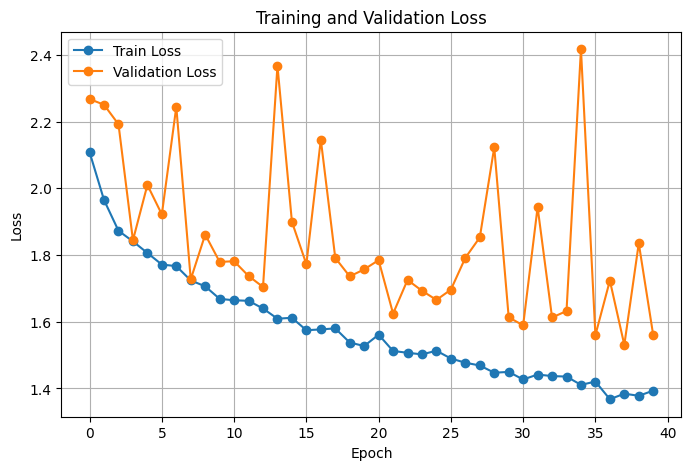
\includegraphics[width=0.8\textwidth]{images/train and validation loss.png}
    \caption{train and validation loss.}
    \label{fig:loss_curves}
\end{figure}


\begin{figure}[H]
    \centering
    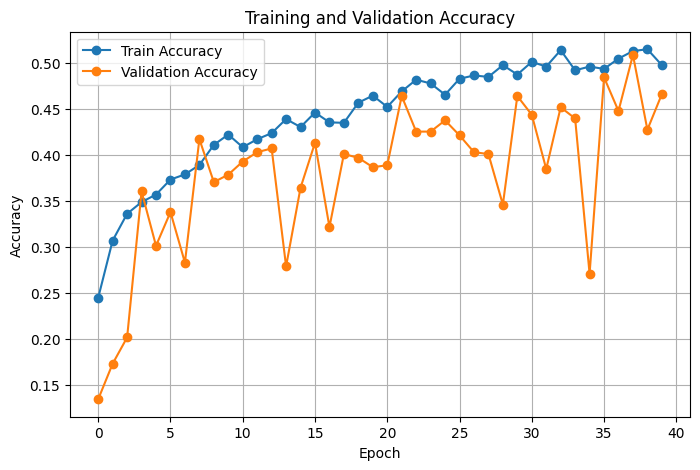
\includegraphics[width=0.8\textwidth]{images/train and val accuracy.png}
    \caption{train and validation accuracy.}
    \label{fig:caccuracy_curves}
\end{figure}





\section{Results and Discussion}

The final model achieved a test accuracy of approximately 50\%.

The macro F1-score was 48.5\%, while the weighted F1-score reached 48.9\%, indicating a moderate classification performance across the ten classes.

The learning curves suggest that the model was still gradually improving during training and did not exhibit severe overfitting. However, the relatively small dataset size and the class imbalance limited the final predictive performance.

The confusion matrix shows that some classes were classified considerably better than others. In particular, classes with a larger number of training examples generally achieved higher recall and precision, whereas minority classes and visually similar categories were more frequently confused.

Despite the moderate accuracy, the results demonstrate that a relatively simple CNN architecture trained on a limited subset of images can still learn meaningful visual representations of garbage categories.

The main objective of this project was not to maximize classification accuracy but rather to develop a fully reproducible computer vision pipeline with reasonable computational requirements and an execution time below one hour on Google Colab hardware.


\begin{figure}[H]
    \centering
    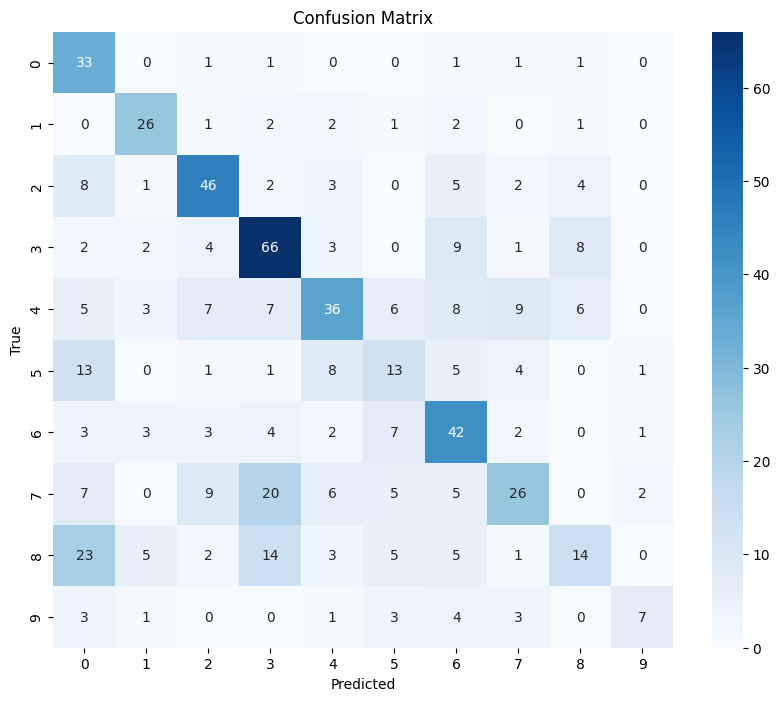
\includegraphics[width=0.8\textwidth]{images/confusion matrix.png}
    \caption{confusion matrix.}
    \label{fig:confusion_matrix}
\end{figure}





\end{document}


